% Overview : 
% put a repository model into cyclus
% that is capable of distinguishing between disposal choices
% and fuel cycle choices
% but is still speedy. 

\begin{frame}[ctb!]
  \frametitle{Methodology : Modularity }
  A modular repository framework facilitates 
  \begin{itemize}
    \item  interchangable subcomponents (e.g. buffer material) so that 
      the impact on the disposal system performance may be observed
    \item and simulations with varying levels of detail.
  \end{itemize}
 \pause
  Integration with a fuel cycle simulator facilitates
  \begin{itemize}
    \item analysis of feedback effects upon the fuel cycle
    \item and investigation of fuel cycle choices on disposal system 
      performance.
  \end{itemize}
\end{frame}

\begin{frame}[ctb!]
  \frametitle{Methodology : Abstraction for Efficiency}

  \begin{minipage}{0.49\textwidth}
      Abstraction simplifies models while capturing salient physics. 
      Parametric analysis with detailed models will inform simpler models at the 
      level of detail important for fuel cycle analysis.
    \begin{figure}[h!]
        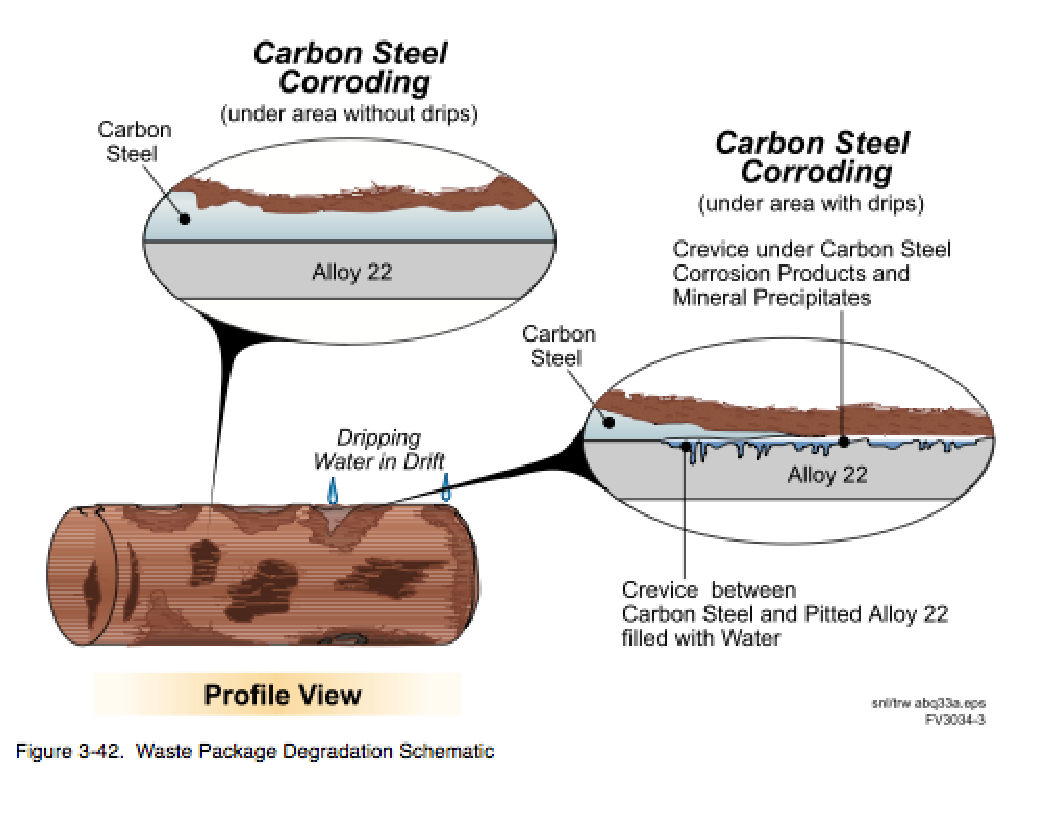
\includegraphics[width=\textwidth]{./images/reality.eps}
      \caption{A complex computational model is an abstraction of reality 
      \cite{doe_viability_1998}.}
      \label{fig:reality}
    \end{figure}
  \end{minipage}
  \hspace{0.01cm}
  \begin{minipage}{0.49\textwidth}
    \begin{figure}[h!]
        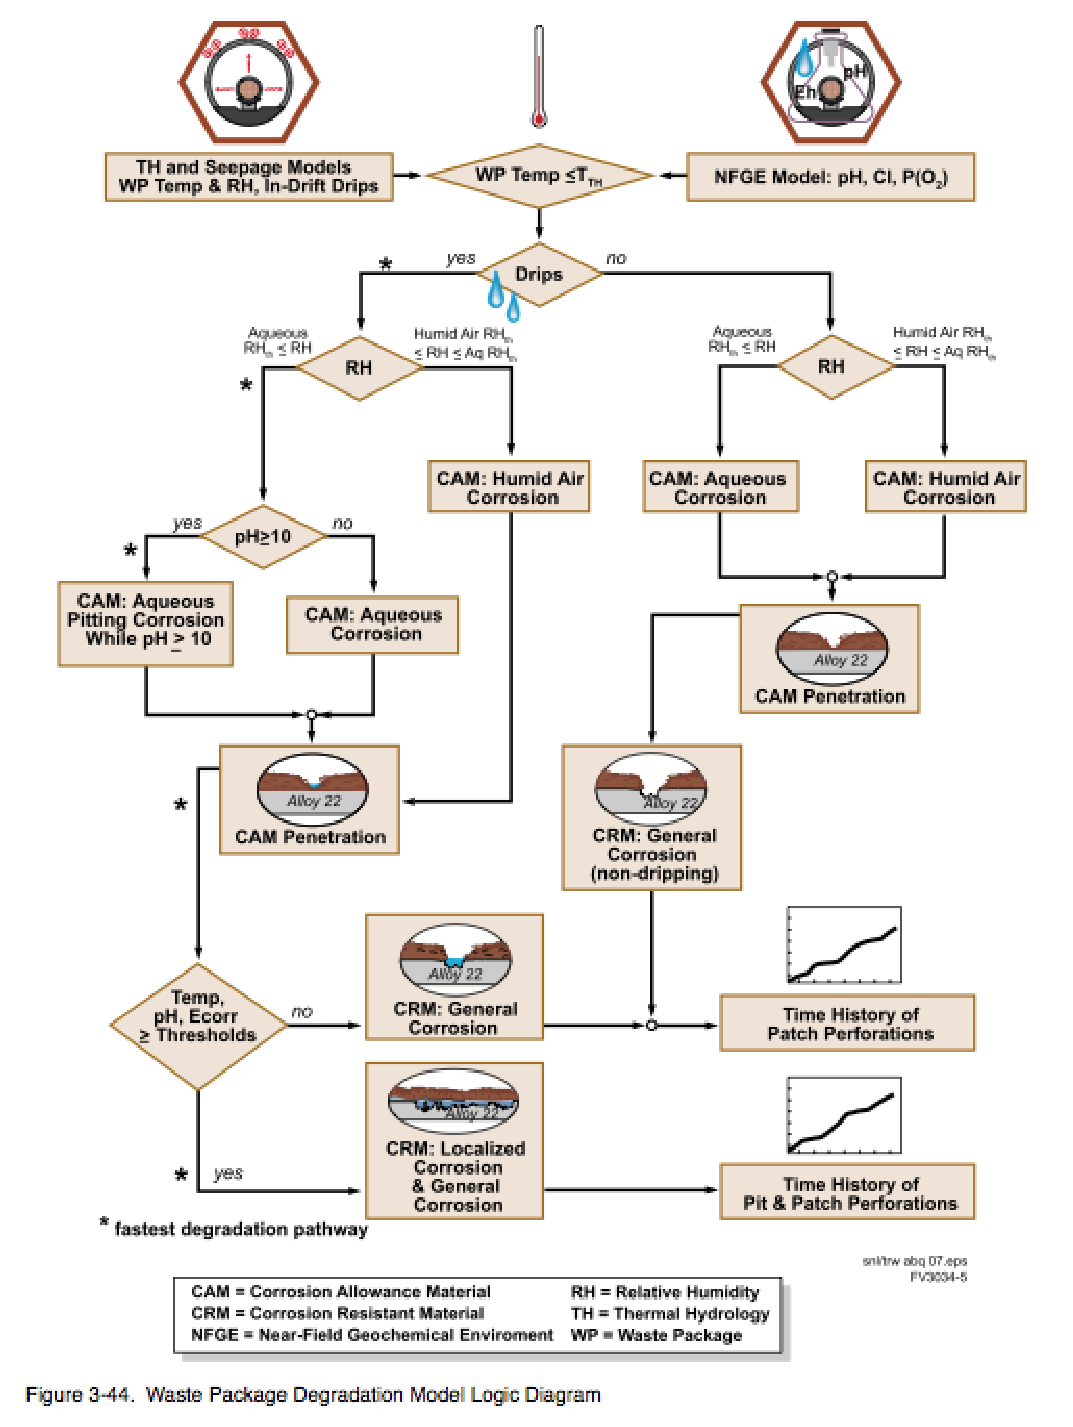
\includegraphics[width=0.9\textwidth]{./images/model.eps}
    \end{figure}
  \end{minipage}
  

\end{frame}
